\osprey 3.0's code has been heavily optimized to improve single-threaded performance relative to the previous version, \osprey 2.2~\cite{COMETS}. Two main areas have received the most attention and the most improvement in performance so far: \as search speed and conformation minimization speed.

\osprey uses the \as search algorithm~\cite{DEE/A*} to perform its combinatorial search over sequence and conformational space~\cite{minDEE,iMinDEE,DEEPer}.  The performance of \as search in \osprey depends mostly on the size of the conformation space of the design: the time required for search scales strongly with the number of mutable and flexible residues. Search time is also dependent on the speed at which we can evaluate the energy scoring functions on \as nodes. Optimizations in \osprey 3.0 have dramatically increased the \as node scoring speed, mainly by caching the results of expensive computations and reusing them at different nodes. Many intermediate values used by the \as scoring functions need only be computed once per design. This reduces the cost of node scoring by roughly an order of magnitude. We can also score child nodes differentially against their parent nodes to speed up node scoring. Caching intermediate values during the parent node scoring and using them to simplify child node scoring yields roughly another order of magnitude speedup in \as node scoring. %\jeff{trying to be concise here, hopefully we don't need the mathematical details of these \as scoring functions?}

\osprey 3.0 also includes optimizations to improve the performance of forcefield evaluation and conformation minimization. Conformation minimization is typically the bottleneck in \osprey calculations with continuous flexibility~\cite{minDEE,iMinDEE,DEEPer,CATS}.  The code in \osprey 3.0 that evaluates forcefield energies for a protein conformation has been heavily optimized, although speed gains here over \osprey2 are modest (roughly two-fold), since the original code was already well-optimized in this area. Much larger performance increases were gained by caching forcefield parameters and lists of atom pairs between different conformations to be minimized, which yielded roughly a 10-fold increase in speed. \osprey 3.0 also increases performance by only evaluating forcefield terms involving mutable and/or flexible residues in a design, since interaction energies between other residues will be identical across all sequences and conformations.  Since most designs only model a minority of the residues in a protein as flexible, this can be a substantial improvement. 

Combined together, these optimizations to single-threaded performance made \osprey 3.0 on average 461-fold faster than \osprey 2.2 (median 28-fold) across 29 protein design test cases, and allowed \osprey 3.0 to finish an additional 16 test cases that \osprey 2.2 could not finish within a 17-day time limit (Fig.~\ref{fig:2v3}, Table~\ref{table:2v3}).  For example, \osprey 2.2 on a Intel Xeon E5-2640 v4 CPU took 49.5 minutes to run a small (6 continuously flexible residues) benchmark sidechain packing problem involving a 114-residue fragment of PDZ3 domain of PSD-95 protein complexed with a 6-residue peptide ligand (PDB ID: 1TP5).  But \osprey 3.0 finished the same design in 7.0 seconds on the same hardware, which is a 424-fold speedup.  

\begin{figure}
\center
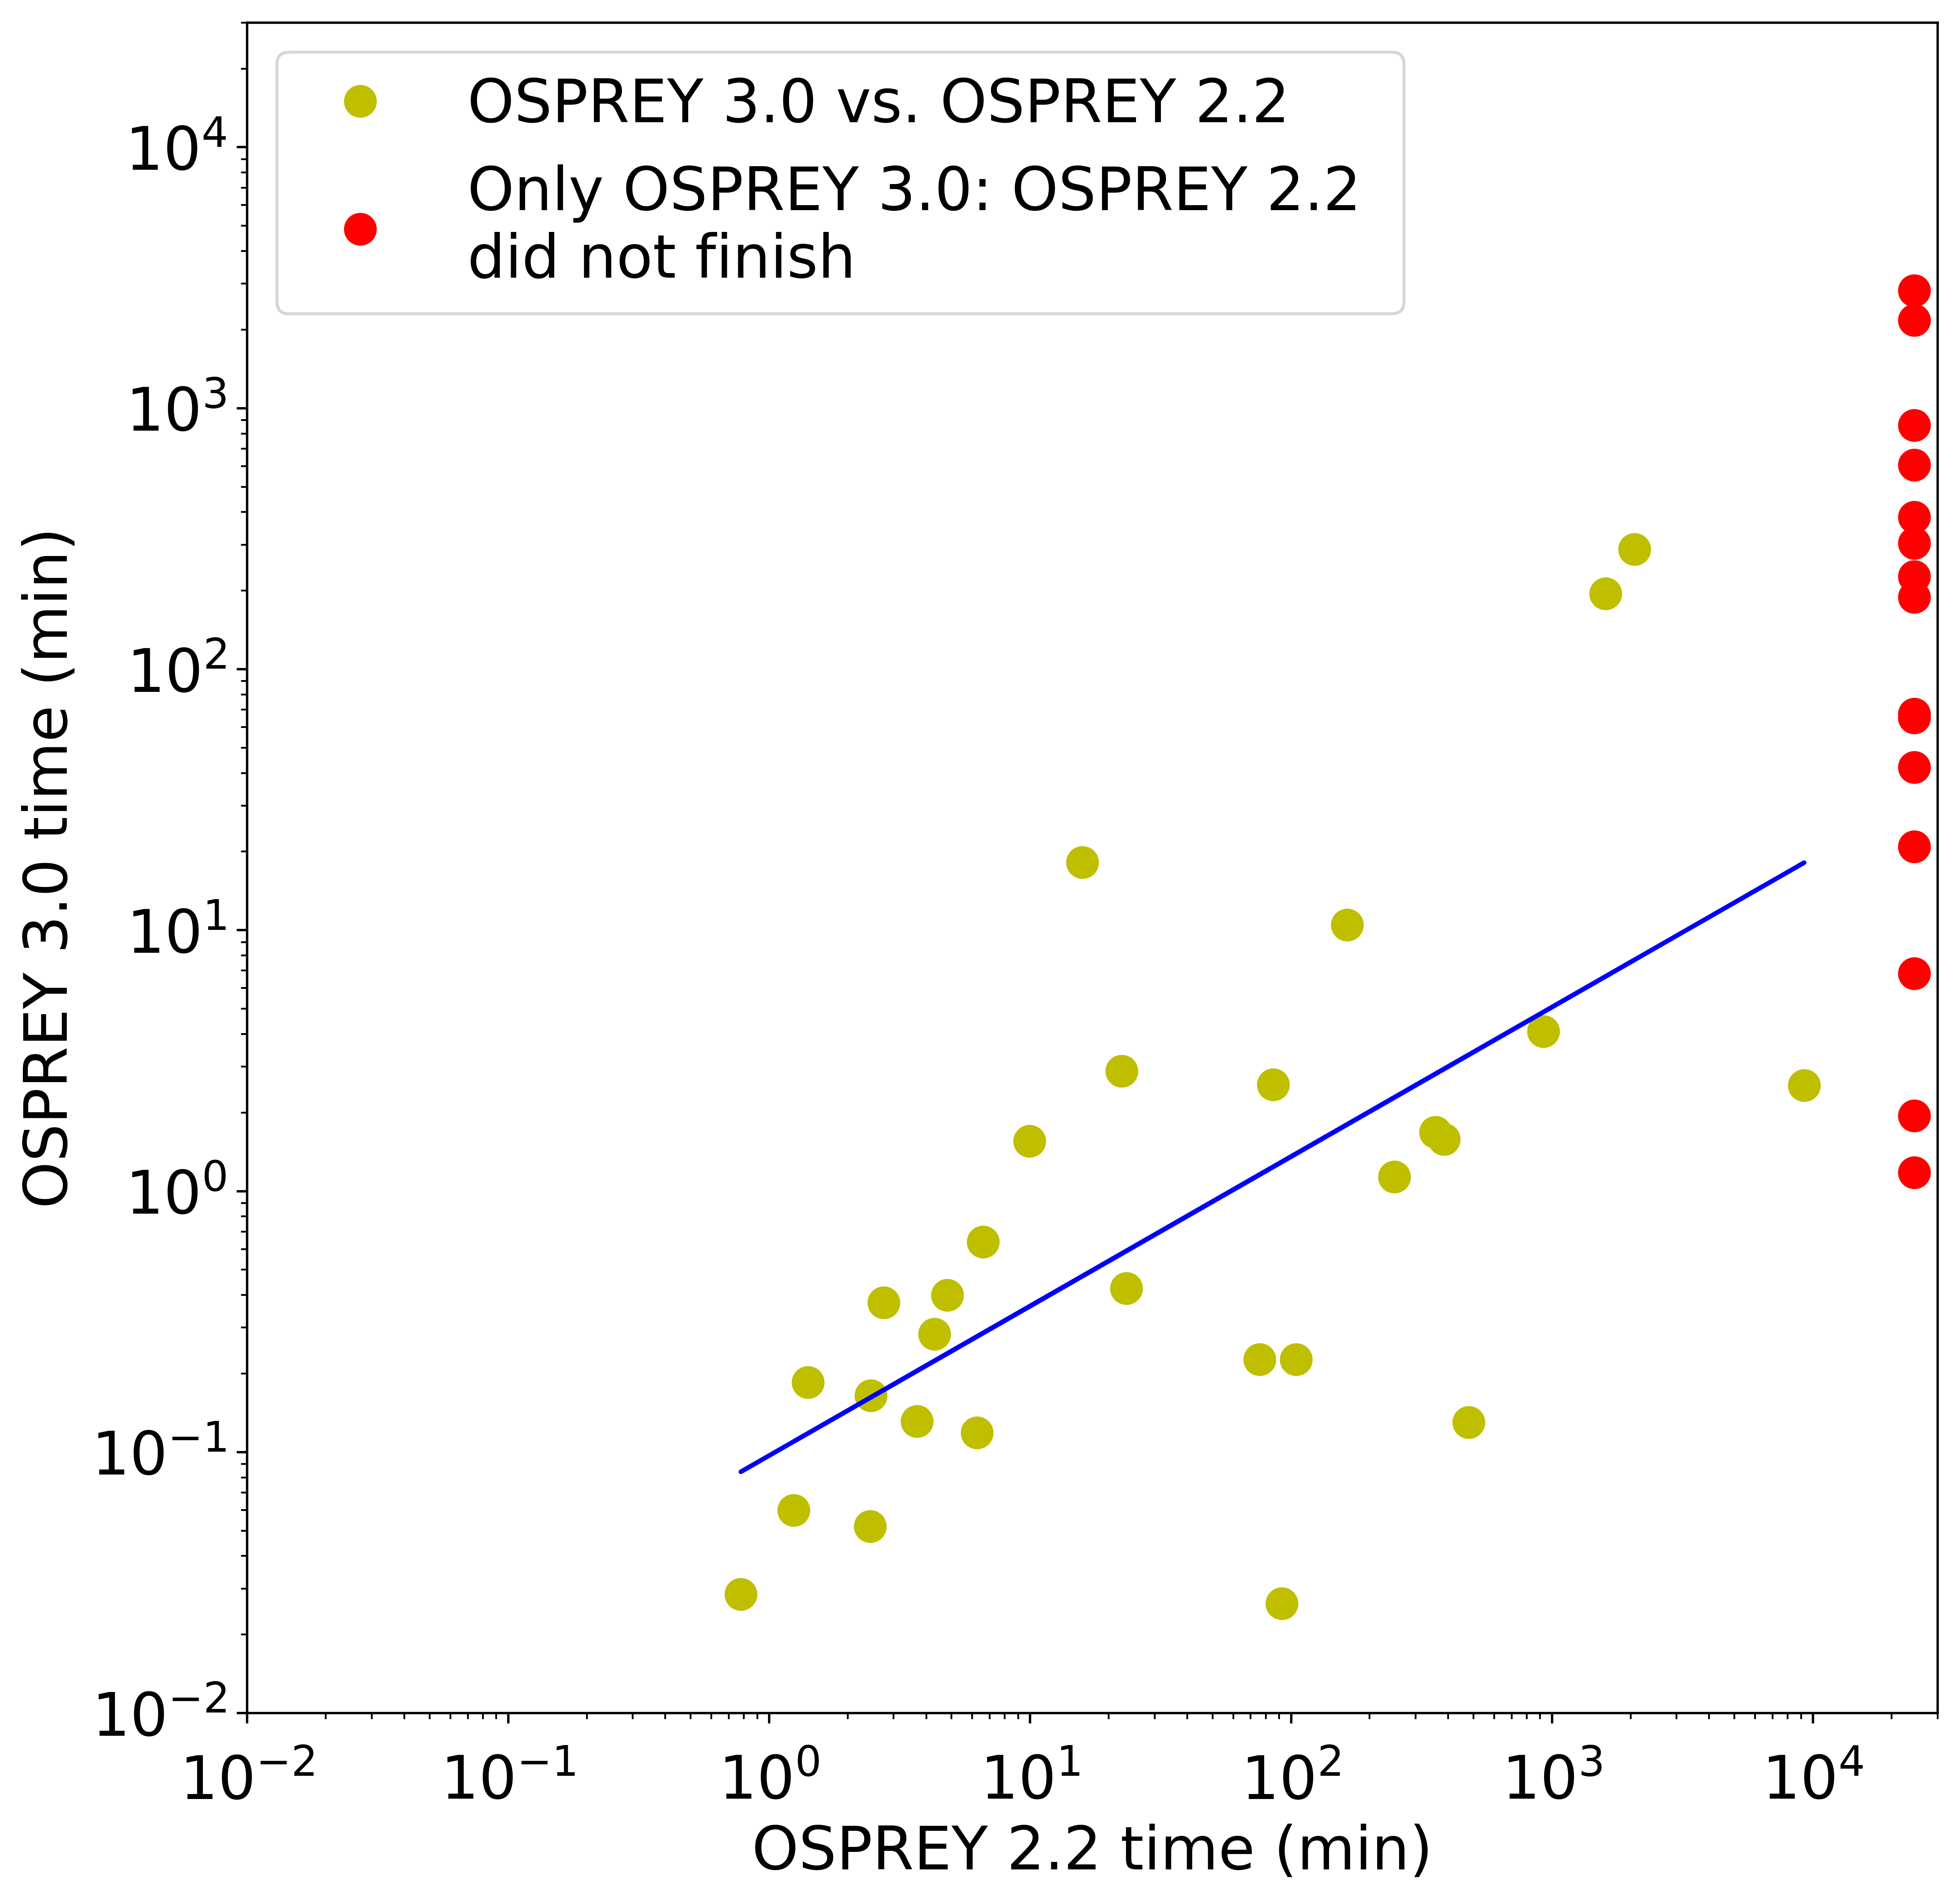
\includegraphics[width=4in]{figures/2v3_times.png}
\caption{Runtimes of \osprey 2.2 and \osprey 3.0 for 45 protein design test cases (details shown in Table~\ref{table:2v3}), shown on a log scale. Designs that only finished with \osprey 3.0 (given a 17-day time limit) are shown on the right in red.}
\label{fig:2v3}
\end{figure}

\begin{table}
\caption{
Details of 45 protein design test cases run on both \osprey 2.2 and \osprey 3.0.  Test cases primarily adapted from Ref.~\citen{EPIC}.  $^a$ Y indicates a partition function calculation (using the $K^*$ algorithm and thus a thermodynamic ensemble of conformations); N indicates calculation of the single global minimum-energy conformation (GMEC). }
\resizebox{\textwidth}{!}{
\begin{tabular}{|p{1.9in}|p{0.5in}|p{0.3in}|p{0.6in}|p{0.75in}|p{0.75in}|p{0.75in}|}
\hline
Protein name	&	PDB code	&	PF?$^a$ 	&	Mutable residue count	&	OSPREY 3.0 time (min)	&	OSPREY 2.2 time (min)	&	Speedup	\\ \hline
Scorpion toxin	&	1AHO	&	N	&	7	&	0.37	&	2.75	&	7.38	\\ \hline
Scorpion toxin	&	1AHO	&	N	&	9	&	0.64	&	6.60	&	10.35	\\ \hline
Scorpion toxin	&	1AHO	&	N	&	12	&	194.71	&	1608.16	&	8.26	\\ \hline
Scorpion toxin	&	1AHO	&	N	&	14	&	287.87	&	2075.04	&	7.21	\\ \hline
Cytochrome c553	&	1C75	&	N	&	6	&	0.28	&	4.30	&	15.19	\\ \hline
Atx1 metallochaperone	&	1CC8	&	N	&	7	&	2.56	&	85.41	&	33.41	\\ \hline
Atx1 metallochaperone	&	1CC8	&	Y	&	7	&	67.12	&	DNF	&	$>$364.72$^\dagger$	\\ \hline
Bucandin	&	1F94	&	N	&	7	&	0.40	&	4.82	&	12.07	\\ \hline
Nonspecific lipid-transfer protein	&	1FK5	&	N	&	6	&	0.03	&	0.78	&	27.34	\\ \hline
Transcription factor IIF	&	1I27	&	N	&	7	&	1.58	&	385.56	&	244.4	\\ \hline
Ferredoxin 	&	1IQZ	&	N	&	9	&	0.16	&	2.45	&	14.92	\\ \hline
Trp repressor 	&	1JHG	&	N	&	7	&	2.88	&	22.50	&	7.8	\\ \hline
Fructose-6-phosphate aldolase 	&	1L6W	&	N	&	6	&	0.23	&	75.97	&	336.22	\\ \hline
Cephalosporin C deacetylase 	&	1L7A	&	N	&	8	&	4.09	&	928.27	&	226.93	\\ \hline
PA-I lectin 	&	1L7L	&	N	&	6	&	0.12	&	6.26	&	52.85	\\ \hline
Phosphoserine phosphatase 	&	1L7M 	&	N	&	7	&	1.13	&	249.33	&	220.11	\\ \hline
alpha-D-glucuronidase 	&	1L8N	&	N	&	5	&	0.13	&	480.13	&	3701.36	\\ \hline
\end{tabular}
}

$^\dagger$ \osprey 2.2 did not finish within the time limit, so we report a lower bound on the speedup: the ratio of the time limit (17 days) to the \osprey 3.0 runtime.   
(Table continues on next page)
\label{table:2v3}
\end{table}

\begin{table}
\resizebox{\textwidth}{!}{
\begin{tabular}{|p{1.9in}|p{0.5in}|p{0.3in}|p{0.6in}|p{0.75in}|p{0.75in}|p{0.75in}|}
\hline
Dachshund	&	1L8R	&	N	&	8	&	0.19	&	1.41	&	7.62	\\ \hline
Granulysin 	&	1L9L	&	N	&	7	&	0.06	&	1.24	&	20.8	\\ \hline
gamma-glutamyl hydrolase 	&	1L9X	&	N	&	5	&	0.03	&	92.13	&	3507.46	\\ \hline
Ferritin 	&	1LB3 	&	N	&	5	&	0.42	&	23.42	&	55.2	\\ \hline
Cytochrome c 	&	1M1Q 	&	N	&	8	&	1.68	&	357.59	&	213.09	\\ \hline
Hypothetical protein YciI 	&	1MWQ	&	N	&	8	&	0.13	&	3.69	&	28.13	\\ \hline
ygfY	&	1X6I	&	Y	&	14	&	604.71	&	DNF	&	$>$40.48$^\dagger$	\\ \hline
ADAR1 ZB domain	&	1XMK	&	Y	&	15	&	2172.23	&	DNF	&	$>$11.27$^\dagger$	\\ \hline
Histidine triad protein 	&	2CS7	&	Y	&	14	&	2816.56	&	DNF	&	$>$8.69$^\dagger$	\\ \hline
Transcriptional regulator AhrC 	&	2P5K	&	Y	&	11	&	1.18	&	DNF	&	$>$20811.61$^\dagger$	\\ \hline
Scytovirin 	&	2QSK	&	N	&	10	&	10.47	&	164.49	&	15.71	\\ \hline
Scytovirin 	&	2QSK	&	Y	&	10	&	2.54	&	9267.19	&	3651.9	\\ \hline
Hemolysin 	&	2R2Z	&	Y	&	12	&	42.02	&	DNF	&	$>$582.58$^\dagger$	\\ \hline
Putative monooxygenase 	&	2RIL	&	N	&	8	&	18.16	&	15.89	&	0.87	\\ \hline
Putative monooxygenase 	&	2RIL	&	Y	&	8	&	0.23	&	104.77	&	463.18	\\ \hline
alpha-crystallin 	&	2WJ5	&	Y	&	15	&	226.32	&	DNF	&	$>$108.17$^\dagger$	\\ \hline
Cytochrome c555 	&	2ZXY	&	Y	&	14	&	381.39	&	DNF	&	$>$64.19$^\dagger$	\\ \hline
High-potential iron-sulfur protein 	&	3A38	&	Y	&	13	&	65.15	&	DNF	&	$>$375.72$^\dagger$	\\ \hline
ClpS protease adaptor 	&	3DNJ	&	Y	&	12	&	65.04	&	DNF	&	$>$376.4$^\dagger$	\\ \hline
Putative monooxygenase 	&	3FGV	&	Y	&	10	&	1.94	&	DNF	&	$>$12591.94$^\dagger$	\\ \hline
Protein G 	&	3FIL	&	Y	&	14	&	303.81	&	DNF	&	$>$80.58$^\dagger$	\\ \hline
Viral capsid 	&	3G21	&	Y	&	15	&	188.53	&	DNF	&	$>$129.85$^\dagger$	\\ \hline
dpy-30-like protein 	&	3G36	&	N	&	4	&	1.55	&	9.97	&	6.43	\\ \hline
dpy-30-like protein 	&	3G36	&	Y	&	4	&	0.05	&	2.44	&	47.07	\\ \hline
Hfq protein 	&	3HFO	&	Y	&	10	&	6.81	&	DNF	&	$>$3594.09$^\dagger$	\\ \hline
Cold shock protein 	&	3I2Z	&	Y	&	14	&	20.84	&	DNF	&	$>$1174.8$^\dagger$	\\ \hline
HPI integrase	&	3JTZ	&	Y	&	14	&	859.69	&	DNF	&	$>$28.48$^\dagger$	\\ \hline
PSD-95 PDZ3 domain	&	1TP5	&	N	&	6	&	0.12	&	49.50	&	424.29	\\ \hline
\end{tabular}
}
\end{table}
